\documentclass[11pt,a4paper]{article}

\usepackage[margin=2.5cm]{geometry}
\usepackage{amsmath,amssymb}
\usepackage{hyperref}
\usepackage[T1]{fontenc}
\usepackage{tikz}
\usetikzlibrary{arrows.meta,positioning}

% Force exact figure placement (prevents floating to later pages/sections)
\usepackage{float}

\title{Context Renormalization:\\
	A Bounded-Memory Protocol for Multi-Session LLM Work}

\author{
	Vasili Gavrilov \\
	\small Independent Researcher
	\and
	ChatGPT\,5.1 \\
	\small Large Language Model
}

\date{}

\begin{document}
	\maketitle
	
	\begin{abstract}
		Collaborations with Large Language Models (LLMs) often span multiple sessions. 
		Over time, these sessions produce design decisions, constraints, and other 
		knowledge that should be carried forward, yet most LLM interfaces impose finite 
		context windows, making naive accumulation infeasible. Furthermore, long 
		interactive exchanges frequently become slow or unstable, because the client 
		interface must maintain an increasingly large DOM tree and conversation 
		transcript. Users are therefore often forced to terminate the session and begin 
		a new one, at the cost of losing accumulated continuity.
		
		This paper introduces \emph{Context Renormalization}, a simple protocol for 
		maintaining a bounded-size ``knowledge ledger'' summarizing essential results 
		of each session. At the end of each session, new information is appended as a 
		delta, and the ledger is compressed back to a fixed text size limit measured in 
		characters. A \emph{Compression Difficulty Score} (CDS) quantifies how hard 
		this compression is, signaling when knowledge should be externalized into 
		permanent documents or implemented in durable artifacts. The protocol is 
		vendor-agnostic: the ledger is plain text, interpretable by any LLM supporting 
		text rewriting. We illustrate the protocol with a two-session design exercise, 
		but the method applies broadly to any multi-session workflow.
	\end{abstract}
	
	\section{Overview}
	
	The protocol relies on a single text file, typically named \texttt{context.txt}, 
	stored with the main project artifacts. This file acts as a bounded, evolving 
	representation of the latent working memory accumulated across multiple LLM 
	interactions.
	
	In real usage, long-running interactions become slow due to large DOM trees, 
	long transcripts, and accumulated UI state. Users often restart the session to 
	regain responsiveness. Context Renormalization allows this safely: before 
	closing the sluggish session, the user requests a ledger update; the next 
	session then begins with the same distilled understanding provided by the ledger.
	
	At each end-of-session boundary, the user provides:
	\begin{itemize}
		\item the current \texttt{context.txt},
		\item any working materials (for example, code snapshots or notes),
		\item and the instruction:
	\end{itemize}
	
	\begin{quote}
		\emph{``End of session. Update context according to the control header protocol.''}
	\end{quote}
	
	The LLM then executes the renormalization algorithm.
	
	% ============================================================
	% SIMPLE, NON-TECHNICAL ILLUSTRATION FOR EARLY READERS
	% ============================================================
	
	\begin{figure}[h]
		\centering
		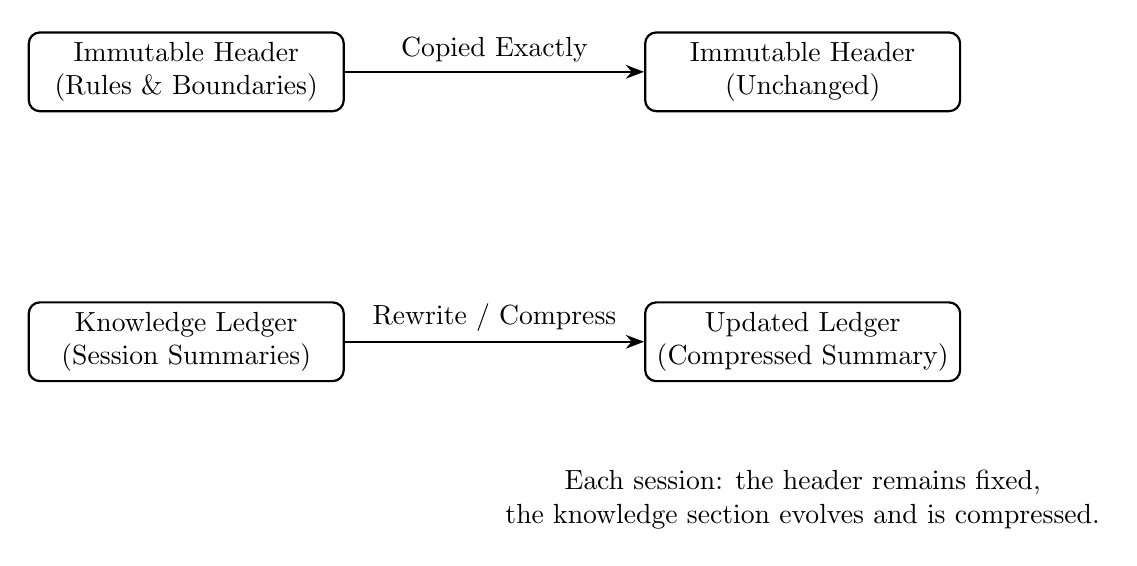
\begin{tikzpicture}[>=Stealth, node distance=2.4cm]
		
		\tikzstyle{box}=[draw, rounded corners, thick, minimum width=4cm,
		minimum height=1cm, align=center]
		
		% Initial header + ledger
		\node[box] (H1) {Immutable Header \\ (Rules \& Boundaries)};
		\node[box, below=of H1] (K1) {Knowledge Ledger \\ (Session Summaries)};
		
		% Next iteration
		\node[box, right=3.8cm of H1] (H2) {Immutable Header \\ (Unchanged)};
		\node[box, below=of H2] (K2) {Updated Ledger \\ (Compressed Summary)};
		
		% Arrows
		\draw[->, thick] (H1.east) -- node[above]{Copied Exactly} (H2.west);
		\draw[->, thick] (K1.east) -- node[above]{Rewrite / Compress} (K2.west);
		
		\node[below=1.0cm of K2, align=center]
		{Each session: the header remains fixed, \\ the knowledge section evolves and is compressed.};
		
		\end{tikzpicture}
		\caption{High-level illustration of Context Renormalization. The immutable header remains unchanged across sessions, while the knowledge ledger is rewritten and compressed to maintain bounded size.}
	\end{figure}
	
	% ============================================================
	% NEW SIMPLE WORKFLOW FIGURE (FOR GENERAL LLM WORK)
	% ============================================================
	
	\begin{figure}[h]
		\centering
		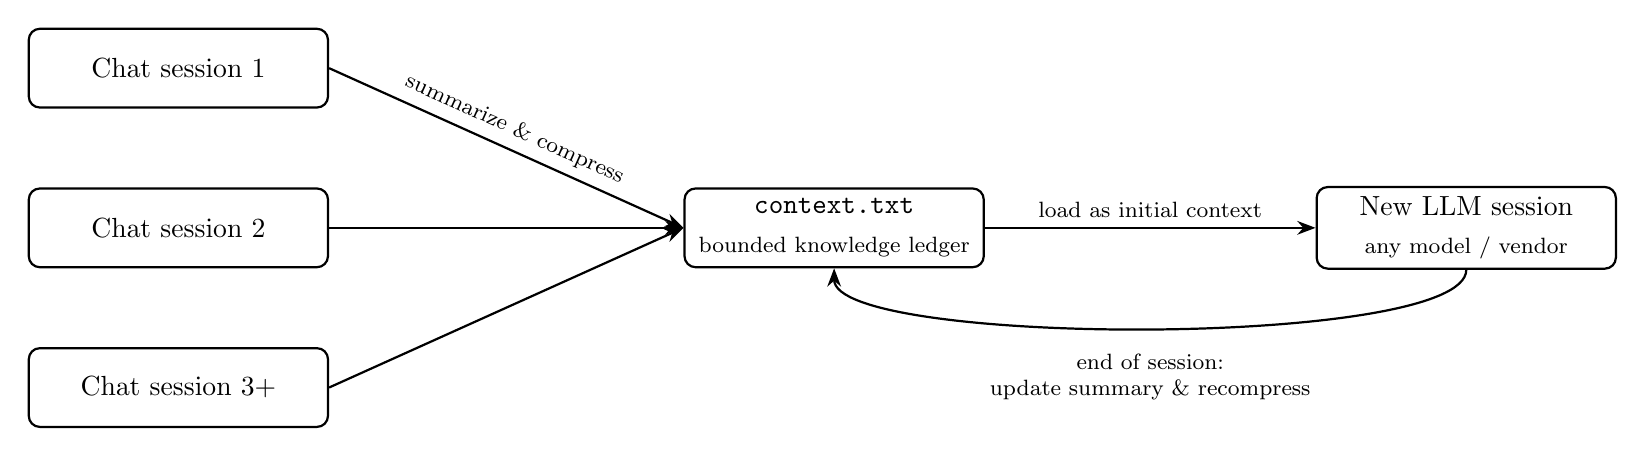
\begin{tikzpicture}[
		>=Stealth,
		node distance=1.8cm,
		box/.style={
			draw,
			rounded corners,
			thick,
			minimum width=3.8cm,
			minimum height=1cm,
			align=center
		}
		]
		
		% Chat sessions on the left
		\node[box] (c1) {Chat session 1};
		\node[box, below=1.0cm of c1] (c2) {Chat session 2};
		\node[box, below=1.0cm of c2] (c3) {Chat session 3+};
		
		% context.txt in the middle
		\node[box, right=4.5cm of c2] (ctx) {%
			\texttt{context.txt}\\[2pt]
			{\footnotesize bounded knowledge ledger}
		};
		
		% New LLM session on the right
		\node[box, right=4.2cm of ctx] (next) {%
			New LLM session\\[2pt]
			{\footnotesize any model / vendor}
		};
		
		% Arrows from chats to ledger
		\draw[->, thick] (c1.east) -- node[above, sloped]{\footnotesize summarize \& compress} (ctx.west);
		\draw[->, thick] (c2.east) -- (ctx.west);
		\draw[->, thick] (c3.east) -- (ctx.west);
		
		% Arrow from ledger to next session
		\draw[->, thick] (ctx.east) -- node[above]{\footnotesize load as initial context} (next.west);
		
		% Recursive update loop (next session back to ledger)
		\draw[->, thick]
		(next.south) .. controls +(0,-1.0) and +(0,-1.0) ..
		node[midway, below=0.2cm, align=center, font=\footnotesize]
		{end of session:\\ update summary \& recompress}
		(ctx.south);
		
		\end{tikzpicture}
		\caption{Workflow of Context Renormalization: multiple chat sessions feed into a compressed ledger (\texttt{context.txt}), which then initializes new sessions and is recursively updated.}
	\end{figure}
	
	% ============================================================
	
	\section{Structure of the Ledger}
	
	\subsection{Control Header}
	
	The control header appears at the top of \texttt{context.txt} and contains:
	\begin{itemize}
		\item \texttt{Session\_Count}: number of summarized sessions,
		\item \texttt{C\_max}: the fixed text size limit (in characters),
		\item the rules of the protocol,
		\item and edit boundaries:
		\begin{verbatim}
		=== BEGIN KNOWLEDGE REGION ===
		=== END KNOWLEDGE REGION ===
		\end{verbatim}
	\end{itemize}
	
	The header is immutable except for incrementing \texttt{Session\_Count}.
	
	\subsection{Knowledge Region}
	
	This is the editable, compressible portion of the file. It consists of 
	chronologically ordered summaries:
	
	\begin{verbatim}
	SESSION 1 --- Summary
	SESSION 2 --- Summary
	...
	SESSION N --- Summary
	\end{verbatim}
	
	Each summary contains durable insights: rules, decisions, invariants, structural 
	clarifications. Ephemeral reasoning is not preserved.
	
	\section{Renormalization Algorithm}
	\label{sec:algorithm}
	
	Let $C_{\max}$ denote the fixed text size limit (in characters). The algorithm proceeds:
	
	\begin{enumerate}
		\item Parse \texttt{context.txt} and increment \texttt{Session\_Count}.
		\item Append a new session summary containing only durable knowledge.
		\item Attempt to compress the knowledge region to remain within $C_{\max}$:
		\begin{itemize}
			\item merge redundant ideas,
			\item rewrite detailed episodes as general rules,
			\item compress older sessions more aggressively,
			\item remove content now encoded directly in project artifacts.
		\end{itemize}
		\item Compute the Compression Difficulty Score:
		\[
		CDS = \max(0, C_{\text{post,min}} - C_{\max}),
		\]
		where $C_{\text{post,min}}$ is the smallest character size achievable 
		without loss of intended meaning.
		\item If $CDS > 0$, include a warning for the user.
	\end{enumerate}
	
	This protocol is fully portable: any LLM capable of text rewriting can apply it.
	
	\section{Compression Difficulty Score}
	
	CDS quantifies representational pressure. It measures how far the final, 
	irreducible text size exceeds the allowed limit:
	
	\[
	CDS = \max(0, C_{\text{post,min}} - C_{\max}).
	\]
	
	Interpretation:
	\begin{itemize}
		\item $CDS = 0$: ledger compresses cleanly; no action needed.
		\item Small $CDS > 0$: mild pressure; consider externalizing knowledge.
		\item Large $CDS$: significant pressure; stabilize knowledge in more durable artifacts.
	\end{itemize}
	
	CDS relates conceptually to description length: it is a practical, operational 
	estimate of the textual complexity of the knowledge state.
	
	\section{Boundedness and Project Phases}
	
	As the session count grows, the ledger must represent more history within the 
	same character limit. Older sessions are compressed into concise statements, 
	but never removed entirely.
	
	At natural project milestones, the ledger can be externalized into permanent 
	documents, and a new ledger can begin with \texttt{Session\_Count = 1}. Thus, 
	the ledger functions primarily as a bounded working memory for an active 
	phase of development, while its compressed snapshots may also serve as a 
	lightweight historical record useful for later analysis, knowledge transfer, 
	or organizational learning.
	
	\section{Cross-Model and Cross-Vendor Use}
	
	The protocol:
	\begin{itemize}
		\item uses plain text only,
		\item does not depend on model-specific memory,
		\item defines its own update rules explicitly in the header.
	\end{itemize}
	
	Therefore, any LLM---regardless of provider or version---can update 
	\texttt{context.txt} as long as it follows the rules. The ledger becomes a 
	portable, model-agnostic mechanism for continuity.
	
	\section{Two-Session Example}
	
	A real design exercise produced a substantial amount of raw dialogue and code. 
	After renormalization with $C_{\max}$ set appropriately, the ledger captured:
	\begin{itemize}
		\item architectural invariants,
		\item structural relationships and rules,
		\item concise summaries of each session,
		\item and no redundant reasoning fragments.
	\end{itemize}
	
	CDS for the first sessions was zero, demonstrating effective compression under 
	the chosen limit.
	
	\section{Related Work and Positioning}
	
	Context Renormalization intersects with several known areas yet differs in 
	important ways.
	
	\subsection*{Conversational Memory and Recursive Summarization}
	
	Work on long-term conversational memory uses recursive or hierarchical 
	summarization to maintain continuity across long interactions. These techniques 
	typically optimize for model performance under finite context windows, whereas 
	Context Renormalization defines a portable, explicit, user-facing ledger with 
	session semantics and a character limit.
	
	\subsection*{Long-Document Summarization and Multi-Stage Compression}
	
	Multi-stage summarization compresses long documents using repeated 
	summarization. Context Renormalization applies a similar idea, but to an 
	evolving project-level knowledge file rather than a static text, and with an 
	explicit rule that older sessions are compressed more aggressively while each 
	session remains represented.
	
	\subsection*{External Memory Systems and Retrieval-Augmented Models}
	
	External memory systems store persistent knowledge in retrievable formats. 
	By contrast, Context Renormalization uses a minimal plain-text ledger requiring 
	no infrastructure, indexing, or retrieval; its portability arises from its 
	simplicity and explicit protocol.
	
	\subsection*{Information Compression and Description Length}
	
	The protocol is conceptually related to minimum description length: the ledger 
	is a bounded textual representation of project knowledge. CDS provides an 
	operational estimate of representational pressure. True Kolmogorov complexity 
	is uncomputable, but the protocol implements a practical, observable 
	approximation by asking the LLM to compress as much as possible without losing 
	essential meaning.
	
	\subsection*{Positioning}
	
	Context Renormalization is not a new summarization algorithm; it is a protocol 
	that combines:
	\begin{itemize}
		\item a fixed-size ledger,
		\item explicit update rules,
		\item fairness across sessions,
		\item and a quantitative compression signal.
	\end{itemize}
	
	It provides a simple, portable method for maintaining continuity across LLM 
	sessions.
	
	% Figure 3: placed at the end of Section 9 and forced to appear HERE (not after Conclusion).
	\begin{figure}[H]
		\centering
		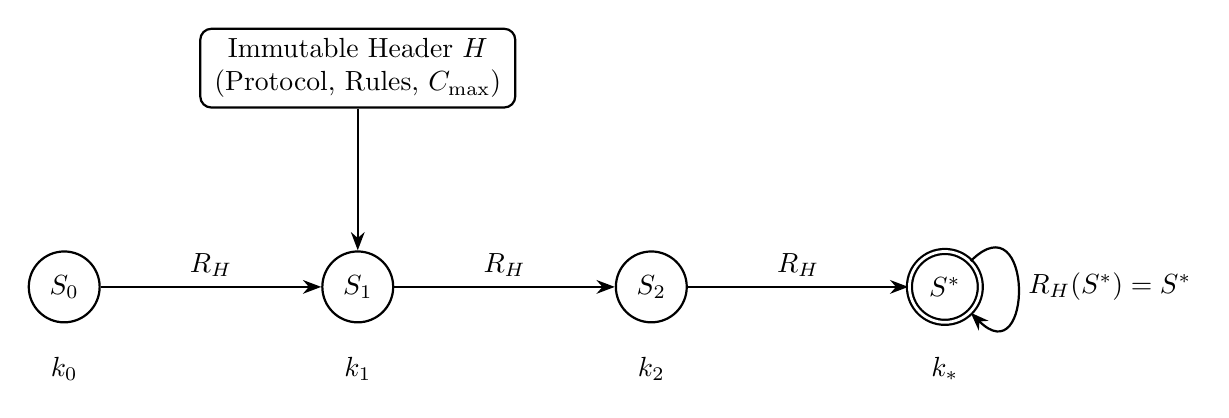
\begin{tikzpicture}[>=Stealth, node distance=2.8cm]
		
		\tikzstyle{state}=[circle, draw, thick, minimum size=0.9cm, align=center]
		\tikzstyle{fpstate}=[circle, double, double distance=1pt, draw, thick,
		minimum size=0.9cm, align=center]
		\tikzstyle{header}=[draw, rounded corners, thick, align=center,
		minimum width=4cm, minimum height=1cm]
		
		% States S_0, S_1, S_2, S*
		\node[state] (s0) {$S_0$};
		\node[state, right=of s0] (s1) {$S_1$};
		\node[state, right=of s1] (s2) {$S_2$};
		\node[fpstate, right=of s2] (sf) {$S^\ast$};
		
		% Scale labels
		\node[below=0.3cm of s0] {$k_0$};
		\node[below=0.3cm of s1] {$k_1$};
		\node[below=0.3cm of s2] {$k_2$};
		\node[below=0.3cm of sf] {$k_\ast$};
		
		% Flow arrows
		\draw[->, thick] (s0) -- node[above] {$R_H$} (s1);
		\draw[->, thick] (s1) -- node[above] {$R_H$} (s2);
		\draw[->, thick] (s2) -- node[above] {$R_H$} (sf);
		
		% Fixed-point loop
		\draw[->, thick] (sf.north east) .. controls +(0.8,0.8)
		and +(0.8,-0.8)
		.. node[right] {$R_H(S^\ast)=S^\ast$}
		(sf.south east);
		
		% Header H
		\node[header, above=1.8cm of s1] (Hnode)
		{Immutable Header $H$ \\ (Protocol, Rules, $C_{\max}$)};
		
		% Influence arrow
		\draw[->, thick] (Hnode.south) .. controls +(0,-0.7) .. (s1.north);
		
		\end{tikzpicture}
		\caption{Renormalization-group view of Context Renormalization. The immutable
			header $H$ defines the operator $R_H$, which maps each compressed ledger
			$S_n$ to its successor $S_{n+1}$. The flow may approach a fixed point
			$S^\ast$ satisfying $R_H(S^\ast)=S^\ast$, representing a stable encoding
			of the project under bounded-memory constraints.}
	\end{figure}
	
	\section{Discussion}
	
	The protocol assumes the LLM can identify redundancy and summarize 
	appropriately. Different models may produce different compression patterns, 
	but the constraints remain stable. Chronic CDS pressure indicates the need to 
	externalize or implement knowledge to maintain boundedness.
	
	Beyond its immediate engineering role, a sequence of compressed ledgers can 
	also be viewed as a historical trace of a particular human--LLM collaboration. 
	Each renormalized context encodes not only technical decisions, but also the 
	approaches, practices, and stylistic patterns that shaped those decisions at 
	a given time. If a project later proves successful relative to comparable 
	efforts, these snapshots may themselves become research artifacts: a compact 
	record of how knowledge, conventions, and design heuristics evolved under 
	bounded-memory constraints.
	
	\subsection*{Organizational Applications}
	
	In organizational settings, a sequence of renormalized contexts can serve as a 
	valuable form of knowledge capture. Each compressed ledger provides a distilled 
	trace of how a particular practitioner interacts with an LLM: their methods, 
	heuristics, strategies of decomposition, and patterns of inquiry. Over time, 
	these traces form a compact representation of an individual's style of work.
	
	Such records may reveal differences in method among collaborators that correlate 
	with effectiveness or creativity. Organizations may analyze these traces to 
	identify best practices, extract transferable techniques, and elevate them into 
	shared standards or onboarding material. In this sense, the ledger supports 
	organizational learning by converting tacit knowledge into explicit form.
	
	Moreover, these preserved traces may surface forms of innovation that would 
	otherwise remain hidden inside unlogged or ephemeral interactions. Many 
	innovative strategies arise not from formal processes but from spontaneous 
	tactics used during day-to-day problem solving. By compressing and preserving 
	these interactions in a structured and comparable form, the ledger makes such 
	tacit experimentation visible. This visibility enables organizations to detect 
	emerging techniques, understand how they differ from conventional practice, 
	and potentially convert them into formalized innovations, training material, or 
	new internal standards.
	
	% ============================================================
	% FUTURE WORK --- METALANGUAGE (TEXT PLUS FORMAL VIEW)
	% ============================================================
	
	\section*{Future Work: A Metalanguage for Recursive LLM Coordination}
	
	Context Renormalization suggests the need for a formal \emph{metalanguage} for
	LLM-to-LLM continuity. The protocol already separates an immutable header---defining
	rules, constraints, and boundaries---from a mutable region that each LLM
	rewrites under bounded compression. This division acts as a meta-level contract:
	the header encodes operational semantics; the ledger encodes evolving state.
	
	Each session constitutes a recursive step: a new LLM receives the immutable
	instructions, transforms the mutable region, and emits a successor ledger. A
	natural research direction is to formalize this process by defining:
	\begin{enumerate}
		\item a typed grammar for the header-language,
		\item machine-checkable invariants for summaries,
		\item forward-compatible rules enabling heterogeneous models to participate,
		\item optional verification that each renormalization obeys the contract.
	\end{enumerate}
	
	Such a metalanguage would make Context Renormalization a general inter-LLM
	coordination mechanism---governing not only what is preserved, but how compression
	and rewriting are interpreted across recursive iterations---thus enabling stable,
	portable continuity across models and vendors.
	
	\bigskip
	
	Formally, each renormalization step can be viewed as the application of an
	operator:
	\[
	S_{n+1} = R_H(S_n),
	\]
	where $H$ is the immutable header defining the rules of the protocol, and
	$S_n$ is the knowledge ledger state after $n$ sessions. The operator $R_H$ is
	fully determined by $H$.
	
	\section{Conclusion}
	
	Context Renormalization supports continuity across multiple LLM interactions 
	under strict size constraints. By combining explicit rules, bounded 
	representations, and a compression difficulty signal, it enables safe session 
	restarts, portability across models, and efficient collaboration.
	
	\appendix
	
	\section{Full Example Ledger (context.txt)}
	Real project ledger produced by multi-session LLM work.
	
	\begin{verbatim}
END OF DAY / UPDATE CONTEXT ACCORDING TO CONTEXT PROTOCOL below
============================================================
CONTEXT PROTOCOL (V2.3 -- IMMUTABLE)
============================================================

Version: 2.3
Context_Session_Count: 4
Context_Total_Budget_Characters: 20000

Purpose / Interpretation:
- This file is a normative rulebook for cross-session continuity.
- It is NOT a tutorial, explanation, or design essay.
- Rules must be concise; do not expand unless explicitly asked.

Global Invariants:
- If a rule, helper, convention, or style exists and is correct, it is canonical.
- Do NOT rewrite, restyle, reformat, or replace canonical material unless explicitly requested.
- Do NOT introduce alternative styles when a canonical one exists.

Optimization Priority:
- Correctness of invariants > cross-session stability > brevity/density.

Update Protocol (MANDATORY):
1) Trigger: user explicitly signals
   "END OF DAY / UPDATE CONTEXT ACCORDING TO CONTEXT PROTOCOL".
2) Read this file fully BEFORE generating output.
3) Increment Context_Session_Count in THIS HEADER ONLY.
4) Append a new block at the END of the KNOWLEDGE REGION named:
   "SESSION <N> -- KNOWLEDGE SUMMARY".
5) Session content MUST include ONLY what is new or changed today.
   Do NOT restate existing rules, code-obvious facts, or prior sessions.
6) If total lines exceed Context_Total_Budget_Characters:
   - Compress older sessions starting from SESSION 1.
   - Remove narrative and redundancy first.
   - Preserve all invariants and decisions.
   - Never delete a session entirely.

Output / Delivery Rule:
- When returning this file, return the ENTIRE FILE
  as plain text inside a single fenced block:
  ```txt <entire file> ```

Knowledge Region Markers (Only lines between the following markers may be edited/compressed):

  - "=== BEGIN KNOWLEDGE REGION ==="
  - "=== END KNOWLEDGE REGION ==="
    @author Vasili Gavrilov 09/12/2025

============================================================
=== BEGIN KNOWLEDGE REGION =================================
============================================================

============================================================
SESSION 1 -- GLOBAL BACKEND, STYLE, REST, DAO, TESTS
(Original "Become the Same Assistant" Context)
============================================================

[1. Global Development Philosophy]
- Goal: minimal entropy; SQL as source of truth.
- No ORMs, no heavy frameworks, no complex routing.
- Java is thin glue:
  - DAO = "SQL + JSON builder"
  - Servlet = "path parsing + auth + call DAO + send JSON"
- No domain POJOs except USER (for login/validation).
- All server responses are JSON; errors are JSON objects with an "error" field.

[2. Core Architectural Pattern]
- Single main servlet: `RestServlet`.
- URL path parsing:
  - `request.getPathInfo()` -> split into segments.
  - Switch on `path.get(0)` (top-level resource).
  - Branch on path length (`n`) and specific suffix segments.
- Examples:
  - `GET /models` -> list models.
  - `GET /models/{id}/runs` -> runs for model.
- Each endpoint block is clearly separated by comment banner:
  - `// ============================`
  - `// /models`
  - `// ============================`

[3. REST Endpoint Design Rules]
- Each endpoint documented in `RESTapi.txt` in this format:
  - `<Object> - <Action>`
  - Path:
  - Client:
  - Server:
  - Errors:
  - Notes:
- `RESTapi-examples.txt` mirrors titles, but contains only curl examples.
- New endpoints require six steps:
  1) Write SQL (debug block first).
  2) Add DAO method.
  3) Add servlet handler.
  4) Add tests in `Tests.java`.
  5) Update `RESTapi.txt`.
  6) Update `RESTapi-examples.txt`.
- No endpoint is "done" until all six steps are complete.

[4. JSON & Naming Conventions]
- JSON field names: lowercase snake_case.
- For single object -> `JSONObject`; for lists -> `JSONArray`.
- Error responses:
  - Always JSON: `{"error":"message"}`.
- No mixing JSON with HTML or other formats.

[5. SQL Style & DAO Pattern]
- SQL is primary design artifact; `create.sql` defines schema.
- Each DAO method:
  1) Starts with commented SQL block for MySQL debugging:

     /*
     SQL for debugging:

     SELECT ...
     FROM ...
     WHERE ...
     */

  2) Java query string built with one clause per line:

     String q =
         "SELECT " +
         "  a, " +
         "  b " +
         "FROM " + schema + "TABLE " +
         "WHERE x = ? ";

  3) Uses `ConnectionProvider.getConnection()`.
  4) Closes `ResultSet`, `PreparedStatement`, and `Connection` in finally.
  5) Returns JSON (never null):
     - `JSONArray` for list results.
     - `JSONObject` for single results; throw NotFoundException if required object not found.
- Avoid redundant checks when SQL already enforces constraints.
- Prefer a single expressive query over multiple round trips.

[6. Authentication Rules]
- Public endpoints:
  - `/status`, `/login`, `/register`, `/users/send_registration`,
    `/password_reset/*`, and static assets.
- All others require auth token:
  - Prefer header: `Authorization: Bearer <token>`.
  - Optional `?token=` query param for GET as fallback.
- Tokens stored in `VALID_TOKEN`.
- Error codes:
  - 401 `{"error":"missing_authentication_token"}`
  - 401 `{"error":"invalid_or_expired_token"}`
  - 401 `{"error":"user_not_found"}`

[7. Testing Conventions (Tests.java)]
- Every endpoint must have a regression test.
- Tests must be DB-idempotent:
  - Insert temporary rows, delete them in finally.
- Typical test flow:
  1) Login to get token.
  2) Call endpoint (via HTTP client).
  3) Check HTTP status.
  4) Check JSON payload structure and important fields.
  5) Cleanup DB rows created by the test.
- Use helper utilities (TestUtil) for:
  - Reading response bodies.
  - Extracting tokens.
  - Deleting test users and tokens.
- Error tests:
  - Check for correct status and error message substring.
- Success tests:
  - Check key fields and array contents.

[8. Core Schema (High-Level)]
- USER: login identity (email), password_hash, timestamps, registration token.
- ROLE, USER_ROLE: authorization; roles include ADMIN, USER, STUDY_ADMIN.
- VALID_TOKEN: active login tokens.
- MODEL_PROVIDER: catalog of model providers (OpenAI, Google, etc.).
- MODEL: specific model versions (e.g., GPT-4), unique by model_name.
- EVAL_SET: named sets of assets (input or output).
- RUN: execution of a model against eval sets (input_eval_set_id, output_eval_set_id).
- ASSET: URI + MIME type, uniquely identified by uri.
- ASSET_SET: eval_set_id <-> asset_id bridge.
- STUDY_TEMPLATE: reusable templates with instructions for studies.
- STUDY: concrete experiment based on template; linked to RUNs via STUDY_RUN.
- SCORE_CARD: aggregated metrics per (study_id, run_id).
- STUDY_TASK_RUN_SCORE: per-task per-run metric values.

[9. Performance Principles]
- Study design (writers) is low-volume; can be slower.
- Study execution (annotators/models) is high-volume; must be optimized.
- Rules:
  - Avoid redundant SELECTs when constraints ensure correctness.
  - Prefer single queries with joins over many small queries.
  - Prefer returning empty arrays over 404 when ID is optional.
  - Use indexes to support common filters (by model_id, eval_set_id, etc.).

============================================================
SESSION 2 -- STUDY / PAGE / QUESTION / ANSWER / ASSET SCHEMA
(Annotation Layer and Page Types)
============================================================

[1. Conceptual Annotation Model]
- Goal: support configurable "study pages" where evaluators see assets
  (e.g., images) and answer questions.
- Key entities:
  - STUDY: experiment configuration.
  - PAGE: one screen in a study.
  - PAGE_TYPE: defines the layout and semantics of how assets and questions interact.
  - ASSET: content item (image/text).
  - ASSET_ON_PAGE: which assets appear on a PAGE.
  - QUESTION: prompt shown on a PAGE.
  - ANSWER: response to a QUESTION in a given STUDY_TASK and RUN.
  - ANSWER_ASSET: per-asset overlay for ANSWER.
  - STUDY_TASK: one participant's run through the study.
  - RUN: model execution, included so model outputs can be evaluated like humans.

[2. The Four Canonical PAGE_TYPE Behaviors]
These types define how questions/answers relate to assets:

Type 1 -- One Asset, Many Questions
----------------------------------
- One asset on the page.
- N questions about that asset.
- Implementation:
  - PAGE: (study_id, page_num).
  - ASSET_ON_PAGE: exactly one asset for that PAGE.
  - QUESTION: many questions for that PAGE.
  - ANSWER: one per (question_id, study_task_id, run_id).
  - Asset can be inferred from PAGE; ANSWER_ASSET optional.

Type 2 -- Many Assets, One Shared Question
-----------------------------------------
- M assets on the page.
- One question applies to all assets (e.g., "average image quality").
- Implementation:
  - PAGE: many assets via ASSET_ON_PAGE.
  - QUESTION: one question on this PAGE.
  - ANSWER: single answer per participant/run.
  - ANSWER_ASSET: one row per asset to mark that this answer applies to each asset.

Type 3A -- Many Assets, Multi-Select (Checkbox)
----------------------------------------------
- M assets on the page.
- One question: "select all that apply".
- Implementation:
  - PAGE: many ASSET_ON_PAGE.
  - QUESTION: single question, type='multi'.
  - ANSWER: one answer per participant/run.
  - ANSWER_ASSET:
    - chosen=1 for each selected asset.
    - chosen=0 or no row for unselected assets (implementation choice).
- Invariant: no upper bound on number of chosen assets.

Type 3B -- Many Assets, Single-Select (Radio)
--------------------------------------------
- Same layout as 3A but exactly one selection.
- Implementation:
  - Same as 3A, but front-end/back-end enforce:
    - Exactly one ANSWER_ASSET with chosen=1 per ANSWER.

Type 4 -- Many Assets, One Question per Asset
--------------------------------------------
- M assets on the page.
- Each asset has its own question (e.g., "Rate image 1", "Rate image 2").
- Implementation:
  - PAGE: many ASSET_ON_PAGE.
  - QUESTION: M questions, each conceptually tied to one asset.
  - Mapping:
    - Either implicit via ordering (question display_order aligns with asset order),
    - Or explicit via QUESTION_ASSET (optional bridge).
  - ANSWER: one per (question, study_task, run).
  - ANSWER_ASSET optional (asset is known via question mapping).

[3. Design-Time Schema Layer]
- PAGE:
  - PK: (study_id, page_num).
  - page_type: FK -> PAGE_TYPE describing which of the four (or future) behaviors.
- ASSET_ON_PAGE:
  - PK: (study_id, page_num, asset_id).
  - Defines which assets appear on each page.
- QUESTION:
  - question_id PK.
  - (study_id, page_num) FK -> PAGE.
  - display_order: natural order on page.
  - type ENUM('text', 'radio', 'multi').
  - UNIQUE (study_id, page_num, display_order) to avoid duplicates.
- Optional QUESTION_ASSET:
  - N<->M association between questions and assets.
  - Minimal version:
    - PK: (question_id, asset_id).
    - FK to QUESTION and ASSET.
  - Only required if:
    - Questions need to reference arbitrary subsets of assets.
    - You want explicit mapping rather than inferring from page_type and ordering.
  - For the 4 canonical types, QUESTION_ASSET can be omitted and logic inferred.

[4. Runtime Schema Layer]
- STUDY_TASK:
  - study_task_id PK.
  - study_id FK -> STUDY.
  - assigned_to FK -> USER.
  - current_page_num, status (ASSIGNED/STARTED/FINISHED), timestamps.
  - Represents one user/model's session in a study.
- ANSWER:
  - answer_id PK.
  - question_id FK -> QUESTION.
  - study_task_id FK -> STUDY_TASK.
  - run_id FK -> RUN.
  - value_text: generic string payload (free text or option key).
  - value_number: generic numeric payload (rating, etc.).
  - UNIQUE (question_id, study_task_id, run_id).
  - Design:
    - ANSWER is strictly per-question, not per-asset.
    - No per-asset flags/values stored here.
- ANSWER_ASSET:
  - PK: (answer_id, asset_id).
  - answer_id FK -> ANSWER.
  - asset_id FK -> ASSET.
  - chosen (boolean) -- used for selection types (3A/3B).
  - per_asset_score (numeric override or per-asset rating if needed).
  - per_asset_text (extra per-asset note if needed).
  - Used for:
    - Type 2: same answer applied to multiple assets.
    - Type 3A/3B: selection of assets.
    - Type 4: optional per-asset customization.

[5. Cardinalities and Invariants]
- STUDY 1 -> N PAGE.
- PAGE 1 -> N QUESTION.
- PAGE 1 -> N ASSET_ON_PAGE (assets on page).
- QUESTION 1 -> N ANSWER (over different study_task/run combos).
- ANSWER N <-> M ASSET via ANSWER_ASSET.
- (Optional) QUESTION N <-> M ASSET via QUESTION_ASSET.
- Session invariants:
  - For each (question_id, study_task_id, run_id), at most one ANSWER.
- Page-type-specific invariants:
  - Type 1: exactly one asset for that page.
  - Type 2/3: multiple assets, exactly one question.
  - Type 3B: per ANSWER, exactly one chosen=1 in ANSWER_ASSET.
  - Type 4: number of questions equals number of assets on that page.

[6. Minimal-Entropy Rules Specific to Annotation Layer]
- ANSWER:
  - Only stores question-level payload: value_text, value_number.
  - No per-asset fields.
- ANSWER_ASSET:
  - Only place for per-asset flags/values (chosen, per_asset_score, per_asset_text).
- QUESTION_ASSET:
  - Optional; drop if you rely strictly on canonical types + ordering rules.
- PAGE_TYPE:
  - Encodes the behavioral semantics.
  - DB schema stores structure; application chooses rendering and logic based on PAGE_TYPE.
- Compression preference:
  - When code encodes a behavior fully (e.g., a newly implemented endpoint),
    context.txt may shrink its narrative description and just document:
    - Purpose,
    - Non-obvious invariants,
    - Any tricky decisions.

[7. How Endpoints Should Expose Annotation Behavior]
- Study-related endpoints should follow global REST patterns:
  - `/studies`, `/studies/{id}`, `/studies/{id}/pages`,
    `/studies/{id}/pages/{page_num}/questions`, `/study_tasks`, etc.
- Read endpoints:
  - Must provide enough info to render one PAGE:
    - page_type
    - list of assets (with URIs)
    - list of questions (with text, type, display_order)
    - any recorded answers for a given study_task/run (value_text/value_number
      and per-asset overlays where applicable).
- Write endpoints:
  - Accept simple JSON (e.g., an array of answers with question_id,
    value_text/value_number, plus optional per-asset selections or scores).
  - Persist into ANSWER, then ANSWER_ASSET accordingly.
- Error and status handling:
  - Follow global conventions from Session 1 (status codes and error JSON).
============================================================
SESSION 3 -- SERVLET ROUTING STYLE + DAILY EXTENSION RULES
============================================================
[1. Mandatory RestServlet Routing Style]
- All REST routing in `RestServlet` must follow the explicit "n-block style".
  This is an architectural invariant and overrides any default ChatGPT style.

- Rules:
  1. Never write compound conditions like:
       if (n == 3 && "pages".equals(path.get(2))) { ... }
  2. Always split by path length first:
       if (n == 1) { ... return; }
       if (n == 2) { ... return; }
       if (n == 3) {
           if ("pages".equals(path.get(2))) { ... return; }
           sendNotFound(...); return;
       }
  3. Every resource section uses the same structure:
       // ============================
       // /studies
       // ============================
       if ("studies".equals(path.get(0))) {
           if (n == 1) { ...; return; }
           if (n == 2) { ...; return; }
           if (n == 3) { ...; return; }
           ... 
       }
  4. Each path.depth (n) forms its own nested block, with its own return.
- Purpose:
  - Matches the existing RestServlet architecture precisely.
  - Ensures no ambiguity in future endpoint additions.
  - Allows developers to visually scan supported path lengths quickly.
  - Eliminates accidental introduction of framework-like routing patterns.

This rule now defines the *canonical* style for all future endpoint additions.

[2. DAO + SQL Style Reinforcement]
- Before any Java query, include a commented SQL block intended for
  copy/paste directly into MySQL CLI.
- Java SQL strings continue to follow the "one clause per line" pattern.
- No multi-query transactions unless explicitly required.

[3. Endpoint Implementation Workflow Reinforcement]
- For each new endpoint:
  1) SQL block (debug-first)
  2) DAO method
  3) Servlet explicit `n-block` handler
  4) Tests.java regression test
  5) Update RESTapi.txt
  6) Update RESTapi-examples.txt

This workflow is required for annotation-layer endpoints such as:
- POST /studies/{id}/pages
- POST /studies/{id}/pages/{page_num}/assets
- POST /studies/{id}/pages/{page_num}/questions
- POST /questions/{id}/assets
- POST /studies/{id}/tasks
- POST /tasks/{task_id}/start
- GET  /tasks/{task_id}/pages/{pageNum}
- POST /tasks/{task_id}/answers
- GET  /tasks/{task_id}/answers
- POST /tasks/{task_id}/finish
============================================================
SESSION 4 -- CANONICAL BACKEND TESTING STYLE (LOCKED)
============================================================
Purpose:
- Define a single, mandatory backend test style.
- Prevent test-style drift, over-abstraction, and helper proliferation.
- This session is normative; deviation requires explicit approval.
Canonical Template:
- `SampleTest.java` is the authoritative test template.
- All backend tests MUST be written by copying and adapting SampleTest.
- SampleTest is a style contract, not a permanent regression test.
Framework Rules:
- JUnit 3 ONLY:
  - `extends TestCase`
  - `public void testXxx() throws Exception`
- Forbidden:
  - `@Test`, JUnit 4/5, parameterized tests, runners, DSLs, new frameworks.
Helper Invariant (Critical):
- IF A HELPER ALREADY EXISTS AND IS CORRECT, IT IS CANONICAL.
- Do NOT rewrite helpers for clarity, style, symmetry, or refactoring.
- Do NOT introduce alternate implementations of existing helpers.
- Example: `TestUtil.read(HttpURLConnection)` must be used as-is.
Allowed Helpers (Strictly Limited):
- `read(HttpURLConnection)` -- existing implementation, unchanged.
- `loginAndGetToken(email, password)` -- optional, for auth boilerplate only.
- Simple JSON accessors (e.g. `getInt(...)`) -- optional.
- Optional minimal DB cleanup helper (e.g. `execUpdate(...)`).
- Explicitly forbidden:
  - response wrapper objects
  - HTTP abstraction layers (`callJson`, etc.)
  - test mini-frameworks
  - hiding HTTP mechanics behind helpers
HTTP Usage in Tests:
- Tests MUST use `HttpURLConnection` inline.
- Each test explicitly:
  - builds URL
  - sets method and headers
  - writes JSON
  - reads status code
  - reads body via `TestUtil.read(...)`
Mandatory Test Structure:
1) Header comment: Endpoint / Case / Expect / Cleanup
2) Arrange
3) Act
4) Assert
5) Cleanup in `finally`
Idempotency:
- Any test that inserts/modifies data MUST clean it up.
- Cleanup must be explicit, local to the test, and in `finally`.
- Tests must be safe to re-run in any order.
Testing Philosophy:
- Tests are specifications, not abstractions.
- Clarity > elegance.
- Duplication is acceptable; hidden behavior is not.
- Optimize for long-term entropy control.
Enforcement:
- Always copy SampleTest.
- Never invent new styles.
- Never refactor helpers unless explicitly requested.
- When unsure, prefer more explicit code, not abstraction.
============================================================
=== END KNOWLEDGE REGION ===================================
============================================================
	\end{verbatim}
	
\end{document}
